\clearpage
\scanpage{3}

A) \uline{Descent and passage to the quotient}

\S\,1\quad Faithfully flat descent

\S\,2\quad \deleted{Passage \unsure{to the|to the} quoti\unsure{ent|.} \unsure{Generalities} on functors on} \inserted{Topologies on $(\mathrm{Sch})_{/S}$. General properties of functors on $(\mathrm{Sch})_{/S}$.} \margin{[Interchange \uline{1} and \uline{2} ??]}
\par\noindent\hfill\deleted{$(\mathrm{Sch})_{/S}$}

\S\,3\quad Passage to the flat quotient.

\S\,4\quad Non-flat descent\quad [\unsure{Application|Applications|Application} : \unsure{Ram.|Rau.|Rem.} Samuel \unsure{generalized} \ldots

\inserted{Application to flatness of a \unsure{schematic} closure and the lemma of \deleted{\unsure{H}}Hironaka.}

\S\,5\quad Passage to the non-flat quotient. [\unsure{Passage} \unsure{to the|to the} \unsure{quotients|quotient} in general]

\S\,6\quad Descent of schemes, relative étale, ----

[\unsure{Év\textsuperscript{t}|Éu\textsuperscript{t}}. descent of étale \deleted{\unsure{morphisms}}\inserted{sheaves} ?? \ldots]

B) \deleted{\uline{General properties of functors on} $(\mathrm{Sch})_{/S}$.}

\figure{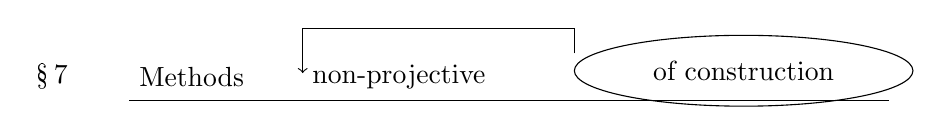
\begin{tikzpicture}[x=1cm,y=1cm]
\node[anchor=west] at (-1.3,0) {\deleted{\S\,7}};
\node[anchor=west] at (0,0) {Methods};
\node[anchor=west] at (2.2,0) {non-projective};
\node (construction) at (7.8,.08) {\inserted{of construction}};
\draw (construction.center) ellipse (2.15cm and .45cm);
\draw[->] (5.65,.3) -- (5.65,.62) -- (2.2,.62) -- (2.2,.05);
\draw (0,-.3) -- (9.65,-.3);
\end{tikzpicture}}

\figure{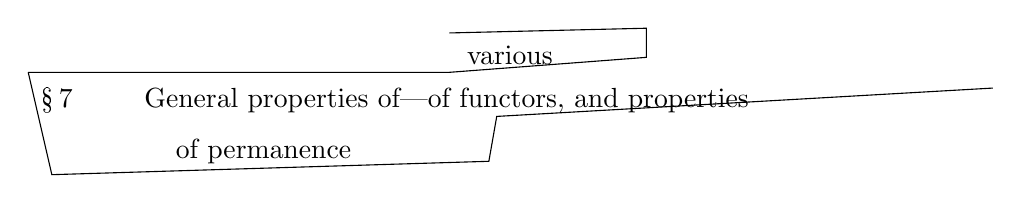
\begin{tikzpicture}[x=1cm,y=1cm]
\node[anchor=west] at (-1.3,0) {\deleted{\S\,7}};
\node[anchor=west] at (0,0) {\deleted{General properties \unsure{of|of} \unsure{functors}, and properties}};
\node[anchor=west] at (.4,-.65) {\deleted{of permanence}};
\node[anchor=west] at (4.1,.58) {\deleted{\inserted{\unsure{various}}}};
\draw (-1.35,.36) -- (4.0,.36) -- (6.5,.55) -- (6.5,.92) -- (4.0,.86);
\draw (-1.35,.36) -- (-1.05,-.94) -- (4.5,-.77) -- (4.6,-.2) -- (10.9,.16);
\end{tikzpicture}}

\S\,7\quad \uline{Prorepresentability}: (and variants).

\tikz[baseline=(p.base),remember picture]{\node[inner sep=1pt] (p) {\S\,\deleted{\unsure{8}}9};}\quad
\inserted{\uline{\unsure{Tangent|Tangent} and normal}} \uline{differential invariants} \deleted{\unsure{of|of the} \unsure{div.}}

\tikz[baseline=(q10.base)]{\node[inner sep=1pt] (q10) {\S\,10};\draw (q10.center) ellipse (1.25em and .9em);}\quad
\margin{\fbox{After \S\,12 ??}}General properties of functors, \uline{permanence properties}
\margin{$\left\{\begin{gathered}\text{\uline{Excellent} functors on S}\\ \text{excellent morphisms}\\ \text{??}\end{gathered}\right.$}

\tikz[baseline=(q11.base),remember picture]{\node[inner sep=1pt] (q11) {\S\,\deleted{\unsure{10|11}}11};\draw (q11.center) ellipse (1.65em and .9em);}\quad
\margin{\tikz[remember picture]{\node[draw,inner sep=2pt] (m11) {\parbox{.90\marginparwidth}{\raggedright Common to \unsure{paragraph} \unsure{20|second|edition} ? Greenberg case ?}};}}
``Elementary'' representabilities of the type $\prod_{\deleted{X}Y/S}X/Y$.

\inserted{cf SGAD $\underline{\overline{\mathrm{VIII}}}$ 6 and $\underline{\overline{\mathrm{XI}}}$ 6.8.}

\tikz[baseline=(r.base),remember picture]{\node[draw,rounded corners,inner sep=1pt] (r) {\S\,8\deleted{\unsure{1|11}}};}
\quad Construction of coherent Modules
\figure{\begin{tikzpicture}[remember picture,overlay]\draw[->] (r.north west) to[out=125,in=190] (p.north);\draw (q11.east) -- (m11.west);\end{tikzpicture}}

\S\,12\quad \deleted{\unsure{Representability}}\inserted{Functors} \unsure{representable} by \inserted{\uline{\unsure{separated|xprés}}} morphisms locally of \unsure{finite|finite} presentation

\S\,13\quad Applications : some relative \unsure{theorem\textsuperscript{s}|theorem\textsuperscript{s}} \deleted{of} representability. (including \unsure{(}for the es étale functors\ldots\unsure{,|)}

% archive sheet number: 2
